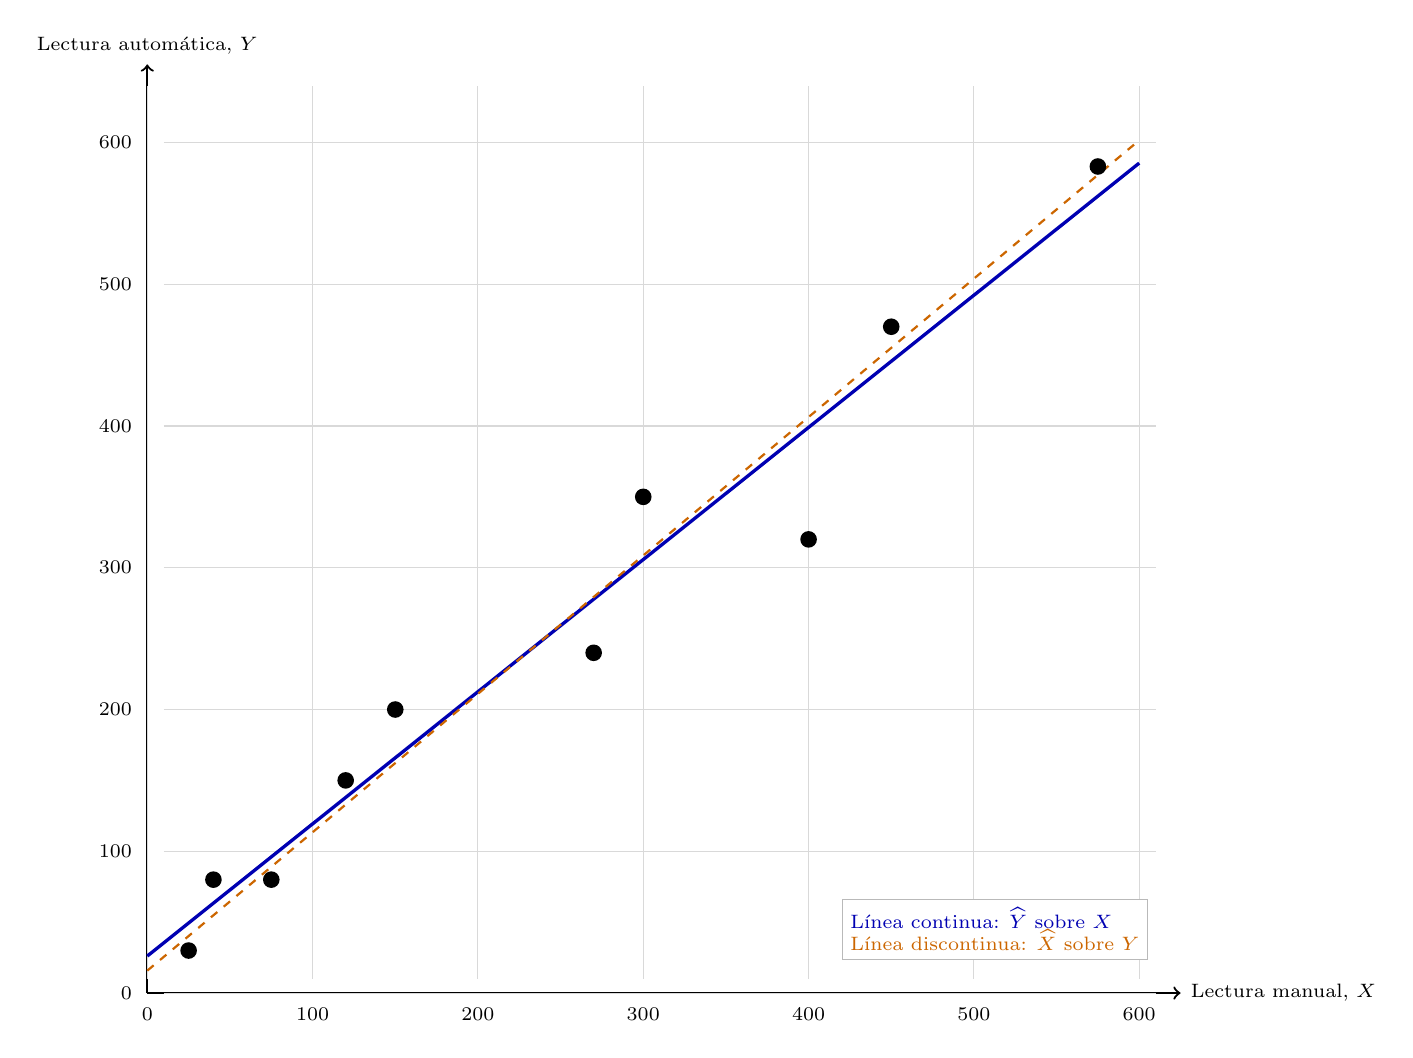
\begin{tikzpicture}[x=0.021cm,y=0.018cm,font=\scriptsize]
    \draw[->,thick] (0,0) -- (625,0) node[right] {Lectura manual, $X$};
    \draw[->,thick] (0,0) -- (0,655) node[above] {Lectura automática, $Y$};
    \foreach \xx in {0,100,200,300,400,500,600} {
        \draw[gray!30] (\xx,10) -- (\xx,640);
        \node[below=2pt] at (\xx,0) {\xx};
    }
    \foreach \yy in {0,100,200,300,400,500,600} {
        \draw[gray!30] (10,\yy) -- (610,\yy);
        \node[left=2pt] at (0,\yy) {\yy};
    }
    \draw[blue!70!black,very thick] (0,26.115) -- (600,585.412);
    \draw[orange!80!black,thick,dashed] (0,15.817) -- (600,601.5);
    \foreach \x/\y in {
        25/30,40/80,120/150,75/80,150/200,300/350,270/240,
        400/320,450/470,575/583
    } {
        \fill[black] (\x,\y) circle (3pt);
    }
    \node[draw=gray!55,fill=white,align=left,anchor=west,inner sep=3pt] at (420,45)
        {\textcolor{blue!70!black}{Línea continua: $\widehat Y$ sobre $X$}\\
         \textcolor{orange!80!black}{Línea discontinua: $\widehat X$ sobre $Y$}};
\end{tikzpicture}